%!TEX root = ../dissertation.tex
\begin{savequote}[75mm]
Nulla facilisi. In vel sem. Morbi id urna in diam dignissim feugiat. Proin molestie tortor eu velit. Aliquam erat volutpat. Nullam ultrices, diam tempus vulputate egestas, eros pede varius leo.
\qauthor{Quoteauthor Lastname}
\end{savequote}

\chapter{Related works}

\section{Phrase Grounding}

Phrase grounding is the task that studies the mapping from noun
phrases to regions of an image (Sec.~\ref{sec:visual-grounding}) and
requires strong understanding of both visual and textual modalities,
specially when not all ground truth is available. 

Even if phrase groudning is an extremely relevant task, the study of
this problem in literature starts relatively late, mostly because a
community-accepted formalization of the problem took its time for
being developed. First efforts in this direction can be identified by
the work of S. Fidler \etal{} \cite{fidler2013sentence}. They
developed a model for semantic understanding of scene exploiting both
textual and visual information. In their work, short sentences are
parsed into nouns and prepositions, which are used to generate
potentials in a holistic scene model. An attempt to find an alignment
between entities in image and sentence is done by C. Kont \etal{}
\cite{kong2014you}. They proposed a model that exploits potentials
computed from text and RGB-D imagery to reason about the class of the
3D objects, the scene type, as well as to align the nouns/pronouns
with the referred visual objects. They used complex sentences, but
grounding is contrained to nouns of 21 object classes relevant to
indoor scenes. In the same period, R. Hu \etal{} \cite{hu2016natural}
moved to a sligtly different task that requires to localize a target
object within a given image based on a natural language query of the
object, named natural language object retrieval. It differs from
text-based image retrieval task as it involves spatial information
about objects within the scene and global scene context. To address
this issue, they proposed a novel Spatial Context Recurrent ConvNet
(SCRC) model as scoring function on candidate boxes for object
retrieval, integrating spatial configurations and global scene-level
contextual information into the network. In particular, their model
processes query text, local image descriptors, spatial configurations
and global context features through a recurrent network, outputs the
probability of the query text conditioned on each candidate box as a
score for the box, and can transfer visual-linguistic knowledge from
image captioning domain to their task. The advent of Flickr30k
Entities dataset collected and processed by B. Plummer \etal{}
\cite{plummer2015flickr30k} (described in Sec.~\ref{subsec:flickr30k})
boosted the development of morea accurate and general models, and
allowed to face the problem phrase grounding without constraints.
Along with the new dataset, they also provided a strong baseline for
phrase grounding based on Canonical Correlation Analysis (CCA) for
phrase grounding task. Their baseline consists in scoring each
region-phrase correspondence separately, without taking into accont
any context of performing any joint inference about the global
correspondence between all regions in the image and all phrases in the
sentence. On the countrary, L. Wang \etal{} in \cite{wang2016learning}
proposed a method for learning joint embeddings of images and text
using a two-branch neural network with multiple layers of linear
projections followed by nonlinearities. The network is trained using a
large margin objective that combines cross-view ranking constraints
with within-view neighborhood structure preservation constraints
inspired by metric learning literature. In
\cite{rohrbach2016grounding}, A. Rohrbach \etal{}, authors developed a
model able to reconstruct textual features in an encoder-decoder
fashion, powered by an attention module which implements localization
of regions of interest. Here, the attention is used to both ground and
reconstruct. During training, the attention learns how to reconstruct
given sentence describing the region to ground. During inference,
attention localizes such region. The key motivation under this idea is
that by training to reconstruct the text phrase, the model learn first
to ground the phrase in the image. Moreover, their model is able to
work with no, semi or full supervision. When no ground truth is
available, the model simply learns to reconstruct the given sentence.
Otherwise, the correct localization is enforced besides the
reconstruction.

As A. Rohrbach \etal{} proved \cite{rohrbach2016grounding}, phrase
grounding problem can be addressed even with some or no ground truth,
allowing, on one side, to learn a more natural approach for grounding,
i.e., wihtout memorizing mapping from phrases to boxes and, on the
other side, to reduce the expansive annotations required with full
supervision. Those annotation, as primarily pointed out by Flickr30k
Entities authors \cite{plummer2015flickr30k} requires a good amount of
work (implying time and money) to be collected because the need of
manual annotators. Large corpus of text and images instead were
already available. Otherwise, even the collection of a new dataset
with shallow information like the link between an image and its
caption is relatively easy to collect. On this wave, many researches
tried to tackle phrase grounding in weak supervised settings.  For
example, F. Xiao \etal{} in \cite{xiao2017weakly} proposed a a
weakly-supervised approach that takes image-sentence pairs as input
and learns to visually ground arbitrary linguistic phrases, in the
form of spatial attention masks. To this end, they introduce an
end-to-end model which learns visual groundings of phrases with two
types of loss functions. In addition to the standard discriminative
loss, which enforces that attended image regions and phrases are
consistently encoded, they propose a novel structural loss which makes
use of the parse tree structures induced by the sentences. In
particular, they ensure complementarity among the attention masks that
correspond to sibling noun phrases, and compositionality of attention
masks among the children and parent phrases, as defined by the
sentence parse tree. Technically speaking, their model encodes a
sentence through a two-layers RNN with LSTM cells and a Dropout model
to prevent overfitting, obtaining $\phi_L(P)$ the language code. The
visual code $\phi_V(I)$ is computed insted by an embedding module,
i.e., a two-layer perceptron with Dropout, that projects features from
VGG-16 convolutional layers to a latent space. Leveragin on weak
annotations their discriminative loss enforces the codes to be similar
when features belongs to linked examples, otherwise to be different.
Formally, given $I_i$ an image and $\{ P^1_i, P^2_i, \ldots, P^n_i \}$
a set of corresponging phrases (both positive and negative), 
\begin{equation}
  L_{disc} = -Y^j_i \cdot Sigmoid(\phi_V(I_i) \cdot \phi_L(P^j_i))
\end{equation}
where $Y^j_i \in \{ -1, +1 \}$ is the indicator variable denoting
whether $P^j_i$ s a negative/positive match to $I_i$. The structural
loss instead heavily exploit relations on sentence structure to
generate an attention mask for localization. A parser first extract
parent-sibling (PC) and sibling-sibling (SIB) relation. Such
constraints are then enforced on the attention mask throught the two
structural loss components $L_{PC}$ and $L_{SIB}$. $L_{PC}$, defined
as 
\begin{equation}
  L_{PC} = \frac{1}{|P|} \sum_{k \in P} \mid A_k - \max_{l \in child(k)} A_l \mid ^ 2,
\end{equation}
tries to bring the attention mask of a parent node and the union mask
of all its children nodes to be close to one another, while
\begin{equation}
  L_{SIB} = - \frac{1}{|S|} \sum_{m \in S} \sum_{pixels \in A} W_m \cdot \log \frac{\max_n A_{m,n}}{\sum_n A_{m,n}}
\end{equation}
introduces competition such that the attention masks of sibling nodes
are exclusive for every pixel.

A few months later, following the idea of attention mask, H. Akbari
\etal{} in \cite{akbari2019multi} addressed the problem of phrase
localization  by learning a multi-level common semantic space shared
by the textual and visual modalities. We exploit multiple levels of
feature maps of a Deep Convolutional Neural Network, as well as
contextualized word and sentence embeddings extracted from a
character-based language model. Following dedicated non-linear
mappings for visual features at each level, word, and sentence
embeddings, we obtain multiple instantiations of our common semantic
space in which comparisons between any target text and the visual
content is performed with cosine similarity. We guide the model by a
multi-level multimodal attention mechanism which outputs attended
visual features at each level. The best level is chosen to be compared
with text content for maximizing the pertinence scores of
image-sentence pairs of the ground truth.

S. A. Javed \etal{} in \cite{javed2018learning} proposed a different
and interesting approach by learning to ground thought a proxy task.
They propose a novel framework for unsupervised visual grounding which
uses concept learning to obtain self-supervision. The intuition behind
this idea is to encourage the model to localize to regions which can
explain some semantic property in the data, such us, the property
being the presence of a concept in a set of images. Basically, given a
set of pairs image and caption all belonging to the same concept, the
model must decode the common concept in the batch. Their model follows
a typical encoder-decoder architecture where the encoder localizes the
region that represents the batch's concept as an heatmap, while
decoder reconstruct the common concept throuhgt a classifier. The
concept batch is constructed by grouping together $k$ pairs image,
caption where all captions contains the same concept. Concept is
extracted from a phrase by selecting all nouns in a phrase thought a
POS tagger and randomly picking one of them.

The idea of using a form of external knowledge is taken up by K. Chen
\etal{} in \cite{chen2018knowledge}, where they approached the problem
by learning to reconstruct the input. However, their approach is
slightly different wrt similar works where the optimization is solely
guided by the reconstruction loss from the language modality. Instead,
it encompasses rich visual information contained in proposals and
useful cues from external knowledge. Their major contributions are
twofold. In order to attend relevant features they introduce the
knowledge base pooling (KBP) gate which returns a score between query
and proposal content computed on the word embedding of proposal
classification label. Basically, they leverage the pretrained object
detector which, along with the proposal, returns a probability
distribution on a vocabulary of labels, used to semantically
categorize the content of the proposal. Such score is computed with a
similarity function (like the cosine similarity) between the word
embeddings of a representative word in query and the proposal class
label. The query representative is computed by averaging the
embeddings of all nouns in the query. Then, they reconstruct both
visual and language modalities. The visual modality is reconstructed
by an attention module that takes embedded features and predicts new
proposal coordinates by optimizing them to be as close as possible to
proposal's. Predicted coordinates as multiplied by the computed
knowledge by KBP gate. The goal of visual consistency branch is to
optimize the attention model via learning to predict location
information contained in query-related proposals. The language
modality is instead reconstructed in a classical way by predicting
thought an RNN with LSTM cells. An high-level overview of the model is
shown in Fig.~\ref{fig:kac-example}.

\begin{figure}
    \centering
    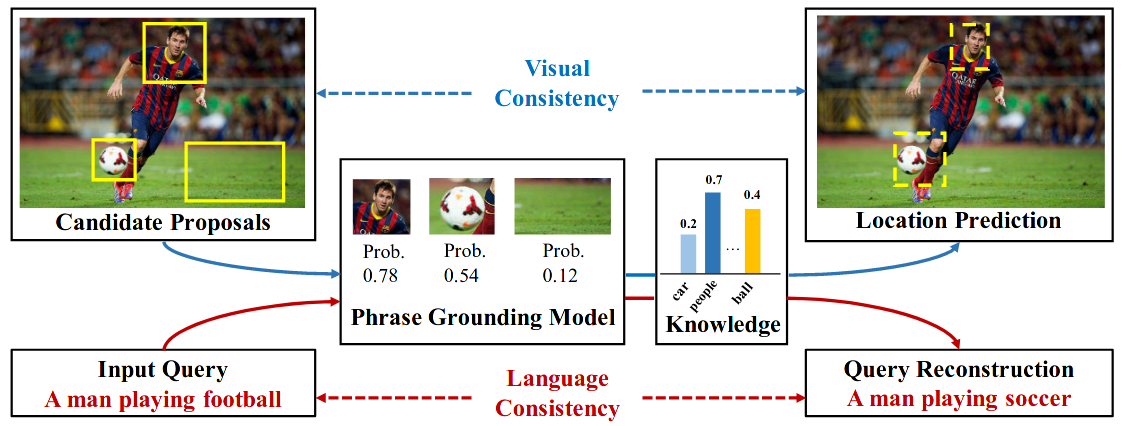
\includegraphics[width=.8\textwidth]{figures/kac-example.png}
    \caption[Knowledge Aided Consistency high-level architecture
    overview]{Knowledge Aided Consistency high-level architecture
    overview \cite{chen2018knowledge}. KAC Net applies both visual and
    language consistency and leverages complementary knowledge from
    the visual feature extractor to facilitate weakly supervised
    grounding.}
    \label{fig:kac-example}
  \end{figure}

In \cite{liu2019adaptive}, X. Liu \etal{} proposed a reconstruction
network based on attention map and optimized for the task of REG
(Sec.~\ref{sec:visual-grounding}). They extract the subject, location
and context features to represent the proposals and the query
respectively. Then, they design the adaptive grounding module to
compute the matching score between each proposal and query by a
hierarchical attention model. Finally, based on attention score and
proposal features, they reconstruct the input query with a
collaborative loss of language reconstruction loss, adaptive
reconstruction loss, and attribute classification loss. The key idea
under their approach is that this adaptive mechanism helps alleviating
the variance of different referring expressions.

\todo{REWRITE papers below}

S. Datta \textit{et al.} in \todo{CITE: align2g} developed three-step
model in which, 
\begin{enumerate*}[label=(\roman*)] 
    \item bounding boxes are filtered based on caption, i.e., only a
    box per caption is selected, then
    \item caption conditioned bounding boxes are encoded with an
    order-invariant deep encoder implemented as a two-layer MLP, and
    finally
    \item those encoded caption-conditioned bounding box are matched
with the caption.
\end{enumerate*}
Tha caption is required to match the encoded features as the model is
optimized for the caption-to-image retrieval proxy task. In the field of weakly-supervised referring
expression grounding, X. Liu \etal{} in \todo{CITE adaptive net}
exploit discriminative information about subject, location and context
wheighted by an attention network and the used to reconstruct the
hidden features of subject, location and context, the input query and
attribute information.

J. Wang in \etal{} \todo{CITE phrase loc}, instead, tried a very new
and different approach. They developed a model able to work under
unsupervised settings, in which no ground truth is available at
training time. The model 
\begin{enumerate*}[label=(\roman*)] 
    \item detects instances by means of six heterogeneous object
    detector, which vary in terms of accuracy, number of classes,
    dataset trained on... then
    \item selects the most related concept with respect to the phrase
    by computing the similarity of detected instance labels and phrase
    words, after this
    \item localized the right bounding box which refers to the
    selected concept.
\end{enumerate*}
The model is not trained: in fact, they leverage the information that
object detector carry with them. A. Rohrbach \etal{} in \todo{CITE
grounding by rec} provide their version of phrase localization in
unsupervised settings together with semi and fully supervised settings
by developing the model \textit{GroundeR}. The model learns to
reconstruct the input phrase based on the boxes it attends to trought
an attention mechanism. 

In supervised settings, the scientific community devoted much effort
solving the phrase localization problem, leading to the development of
many solution making use of different strategies. 
Z. Yang \etal{} in \todo{CITE a fast and acc one stage
appr} exploit YOLOv3 object detector features joined with textual
features in order to learn to ground wihtout requiring the proposal
extraction stage. In \todo{CITE zero shot groudning}, A. Sadhu \etal{}
on the same line of \todo{CITE a fast and acc one stage appr} propose
a one-stage model focusing on the slightly different task of Zero Shot
Grounding, which can include unseen nouns in phrases. Instead, D.
Rigoni \etal{} in \todo{CITE a better loss} optimize the model to
learn with a new loss involving the use of metrics like Intersection
Over Union (IoU) and Complete IoU (CIoU).

\newthought{Visual Textual Knowledge Entity Linking}, introduced in
\todo{CITE 10, 8, 9 da a new loss}, is a more complex task than phrase
localization: it requires an artificial agent to jointly recognize the
entities shown in the image and mentioned in the text, and to link
them to its prior background knowledge. The solution to the VTKEL
problem could lead to major scientific advancement towards a better
understanding of semantic information contained in the image and
textual sentence, respectively. In fact, the knowledge graph allows to
introduce semantic reasoning on the information contained in both the
image and the textual sentence, which could lead to innovative
solutions for the weakly supervised phrase localization problem and
for the partially annotated dataset problem.

\newthought{Visual Question Answering} (VQA) is a computer vision task
where a system is given a text-based question about an image, and it
must infer the answer \todo{CITE VQA future chal}. Questions can be
arbitrary and can encompass many computer vision task, varying from
object recognition or detection to attribute or scene classification
and also to counting. Beyond this, there are many more complex
question that can be asked, such as questions about spatial
relationships among objects and common sesnse reasoning question. 
Under this definition, phrase localization becomes a foundamental
building block for VQA systems.

\todo{ image retrieval ??? altro? }
